\documentclass[a4paper,oneside]{book}
\usepackage[backend=biber,natbib=true,style=authoryear]{biblatex}
\addbibresource{~/1_PROJECTS/GitHub/math-lecture-notes/NQBH_Bibliographies.bib}
\usepackage[utf8]{inputenc}
\usepackage{graphicx}
\usepackage{subfigure}
\usepackage[colorlinks=true,linkcolor=blue,urlcolor=red,citecolor=magenta]{hyperref}
% Math
\usepackage{amsmath,amssymb,amsthm}
\allowdisplaybreaks
\numberwithin{equation}{section}
\newtheorem{assumption}{Assumption}[section]
\newtheorem{lemma}{Lemma}[section]
\newtheorem{corollary}{Corollary}[section]
\newtheorem{definition}{Definition}[section]
\newtheorem{proposition}{Proposition}[section]
\newtheorem{theorem}{Theorem}[section]
\newtheorem{notation}{Notation}[section]
\newtheorem{remark}{Remark}[section]
\newtheorem{example}{Example}[section]
\newtheorem{ques}{Question}[section]
\newtheorem{problem}{Problem}[section]
\newtheorem{conjecture}{Conjecture}[section]
% Layout
\usepackage[left=0.5in,right=0.5in,top=1.5cm,bottom=1.5cm]{geometry}
% Header & Footer
\usepackage{fancyhdr}
\pagestyle{fancy}
\fancyhf{}
\addtolength{\headheight}{0pt}% obsolete
\lhead{\itshape \small \chaptername~\thechapter}
\rhead{\itshape \small \nouppercase{\leftmark}} %\nouppercase !
\renewcommand{\chaptermark}[1]{\markboth{#1}{}}
\cfoot{\thepage}
\usepackage{color}
\usepackage[table]{xcolor}
\definecolor{light-gray}{gray}{0.7}
\definecolor{dark-gray}{gray}{0.4}
\definecolor{orange}{rgb}{1,0.5,0}
%
\definecolor{dgreen}{rgb}{0.,0.6,0.}
\definecolor{dred}{rgb}{0.6,0.,0.}
\definecolor{dorange}{rgb}{0.9,0.5,0.}
\definecolor{dblue}{rgb}{0.,0.,0.6}
\definecolor{grey}{rgb}{0.5,0.5,0.5}
 

\title{\begin{figure}
        \begin{center}
            
\includegraphics[width=\textwidth]{head.jpg}
        \end{center}
    \end{figure}
    Handbook for Software:\\
    Shape- and Topology Optimizations
    \begin{figure}[b]
        \begin{center}
            \subfigure{
                
\includegraphics[width=3.5cm,height=1.38cm]{HU.jpg}}
            \subfigure{
                
\includegraphics[width=3.5cm,height=1.38cm]{empty.jpg}}
            \subfigure{
                
\includegraphics[width=2.5cm,height=1.38cm]{empty.jpg}}
            \subfigure{
                
\includegraphics[width=1.69cm,height=1.19cm]{ifb.jpg}}
        \end{center}
    \end{figure}}
\date{\today}

\begin{document}
\maketitle

\setcounter{secnumdepth}{4}
\setcounter{tocdepth}{4}

\tableofcontents

\chapter*{Authors}

\begin{itemize}
    \item Prof. Dr. M. Hinterm\"uller (Humboldt-Universit\"at zu Berlin)
    \item Dr. K. Knall (Mathtec, Wien)
    \item MMag. M. Kanitsar (Mathtec, Wien/Universit\"at Graz).
\end{itemize}

\chapter{Installation}

\section{Folder structuring and compilation of the applications}
To use the shape and topology optimizations, the standard installation of OpenFOAM \verb|$FOAM_APP/solvers/incompressible/| must be extended by the following applications:
\begin{itemize}
    \item \texttt{generateFieldsFoam}
    \item \texttt{shapeGradientWall}
    \item \texttt{shapeGradientCCM}
    \item \texttt{setupShapeGradientCCM}
    \item \texttt{shapeGradientAddSTL}
    \item \texttt{shapeGradientCloseAll}
    \item \texttt{topoOpt}
    \item \texttt{topoOptCloseAll}
    \item \texttt{topoExtractSTL}
\end{itemize}
The folder \texttt{InitialSGccm} must be copied into the \verb|$FOAM_RUN/tutorials/| directory. The console commands for installation can be found in the shell-script \texttt{installShapeGradient.sh}.

%------------------------------------------------------------------------------%

\chapter{Geometry Data}

\section{Storage structure of the data in STL format}
The geometry data must be created in the \verb|initial_stl| folder. In addition to the installation space geometry (\texttt{bds.stl}), the surfaces are saved in 4 files in STL format (\texttt{inlet.stl}, \texttt{fixed.stl}, \texttt{wall.stl}, \texttt{outlet.stl}).

The test geometry \textit{M23} with 2 inlets, 3 outlets and an additional fixed geometry (see Table \ref{tab:stlData1}) serves as an illustration.

\begin{figure}[htbp]
    \centering
    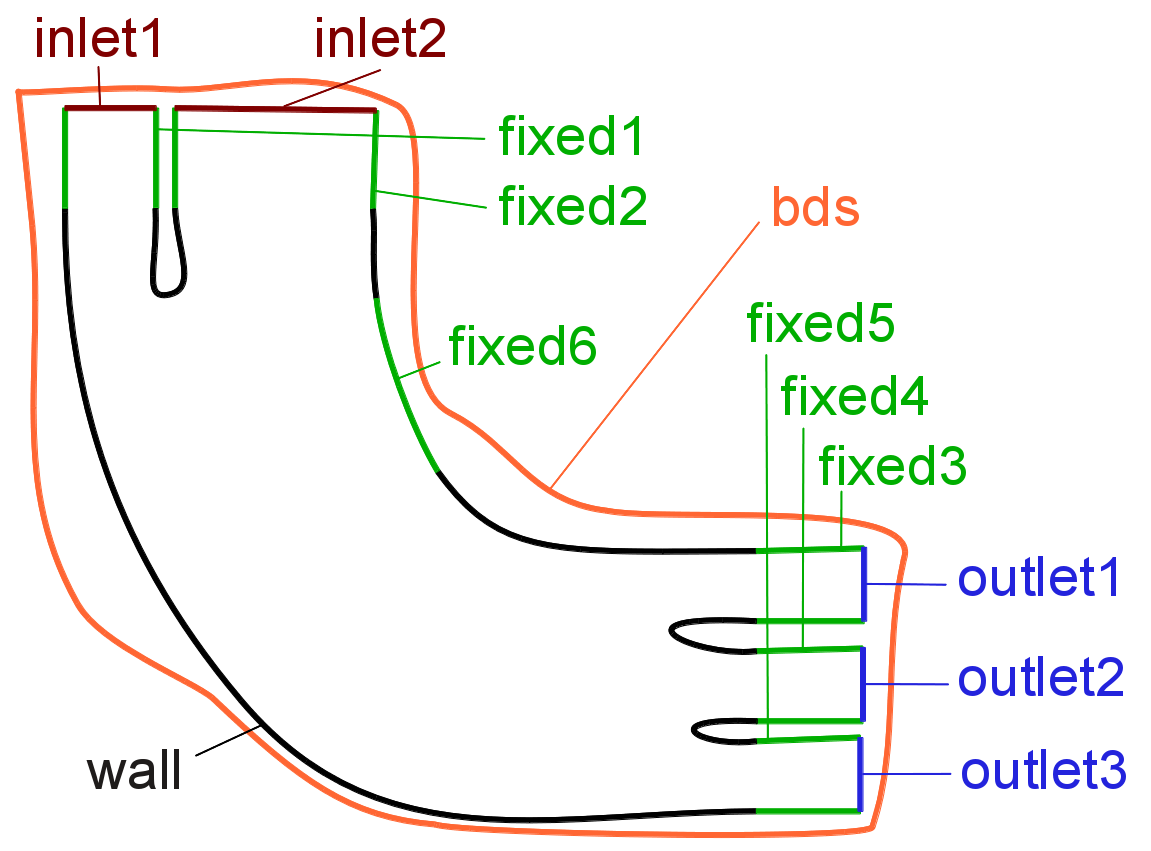
\includegraphics[scale=0.55]{skizze_designSpace4.png}
    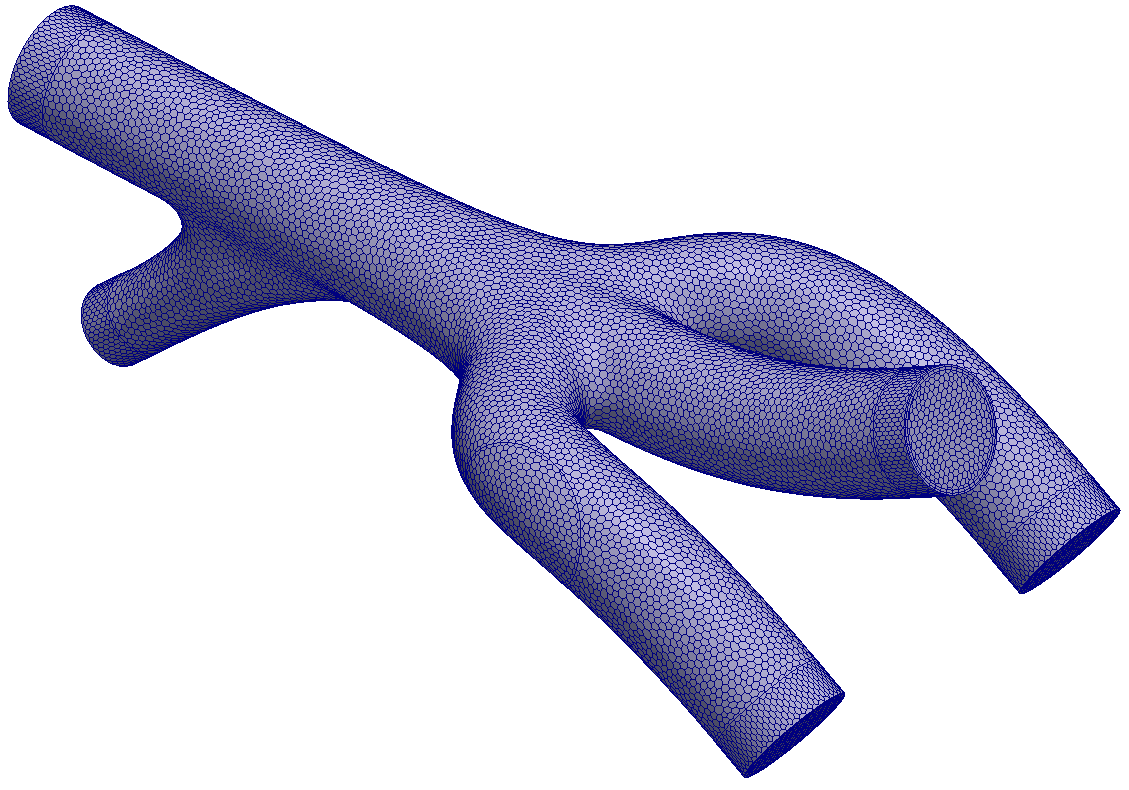
\includegraphics[scale=0.18]{M23all.png}   
    \caption{Left: Sketch geometry data, right: test geometry M23.} 
    \label{fig:sketch building space}
\end{figure}
Each inlet and outlet area has a fixed geometry that describes the connection to the geometry to be optimized. Additionally, the user can define fixed geometries which are only connected to the geometry to be optimized (e.g.: \texttt{fixed6} in test geometry \textit{M23}).

The fixed geometries are numbered consecutively, starting with the connections to the inlet geometry, continuing with the connections to the outlet geometry and ending with the fixed geometries that are only connected to the geometry to be shape optimized.

When selecting the installation space geometry, care should be taken to ensure that the start geometry is completely within the allowed range and extends beyond the \verb|inti_freegeom_fixed-inlet| and \verb|into_free-geom_fixed-outlet| interfaces (see Fig. 2.1).

\begin{table}[!htbp]]
    \centering
    \begin{tabular}{|c|p{8cm}|c|c|} %lcrp
        \hline
        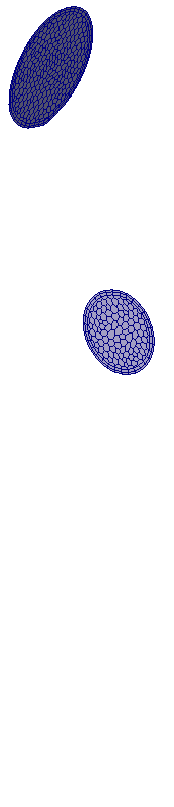
\includegraphics[scale=0.4]{M23in.png} & 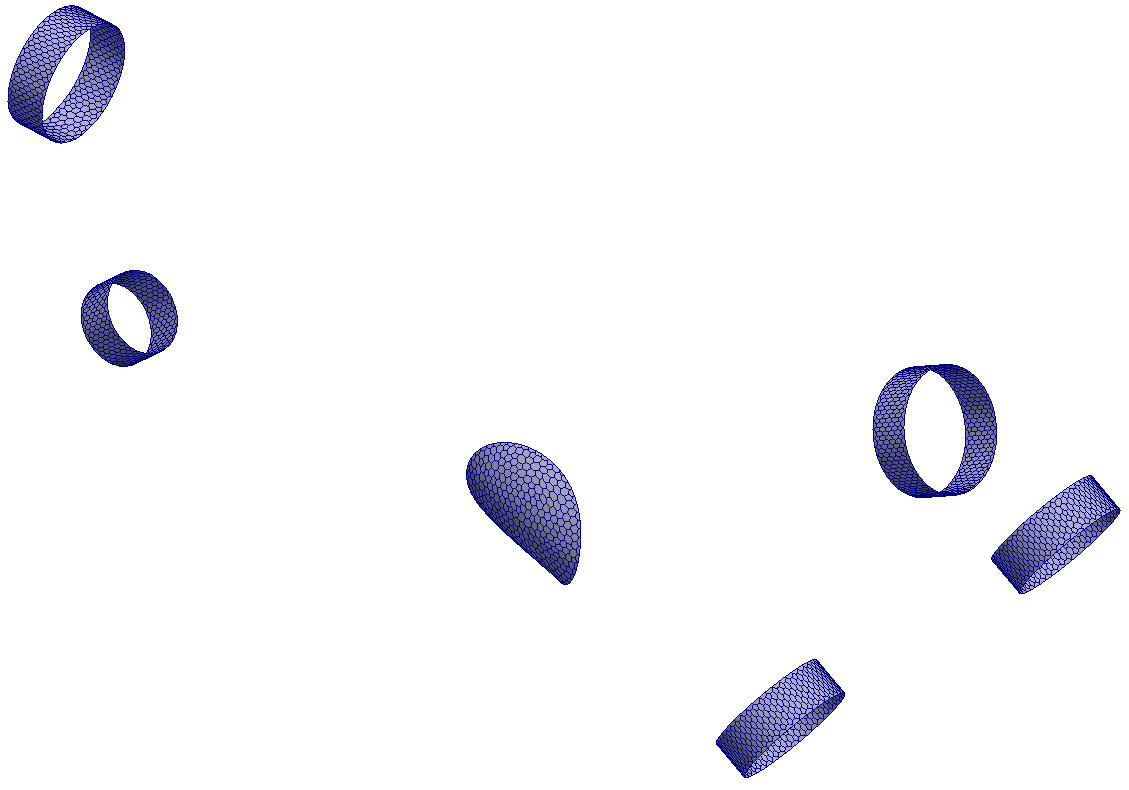
\includegraphics[scale=0.1]{M23fixed.png} &   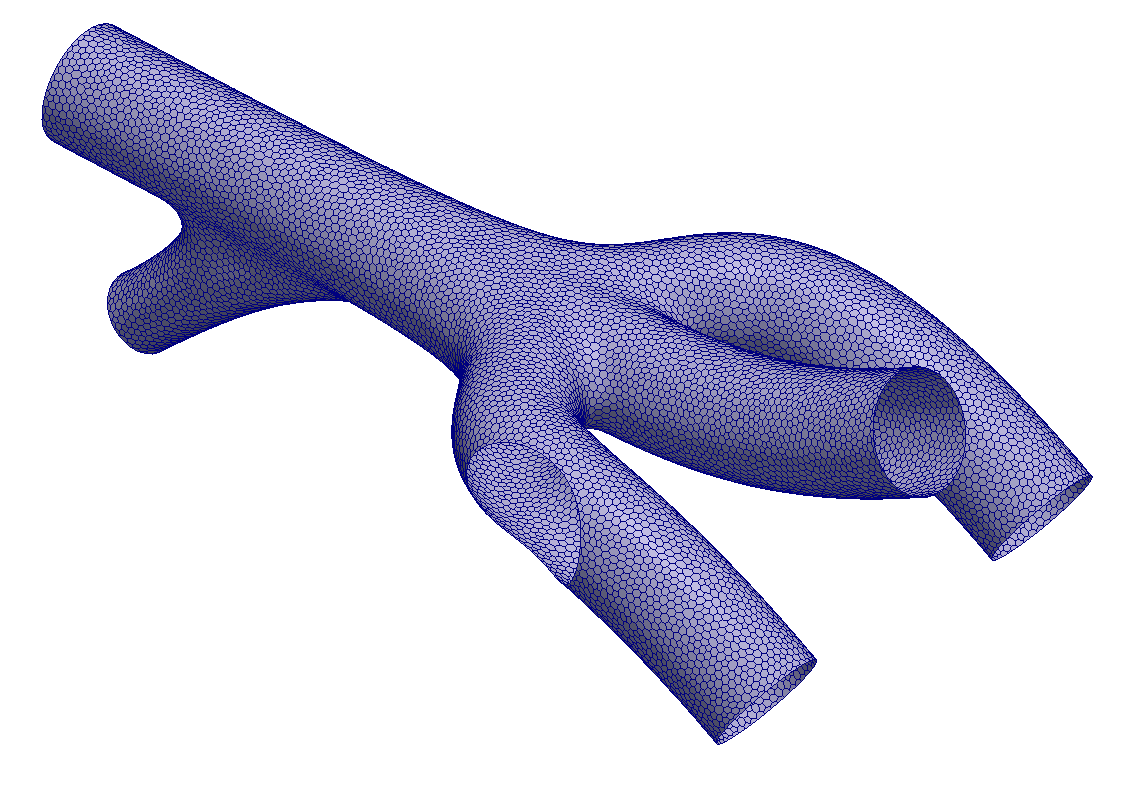
\includegraphics[scale=0.1]{M23wall.png} &   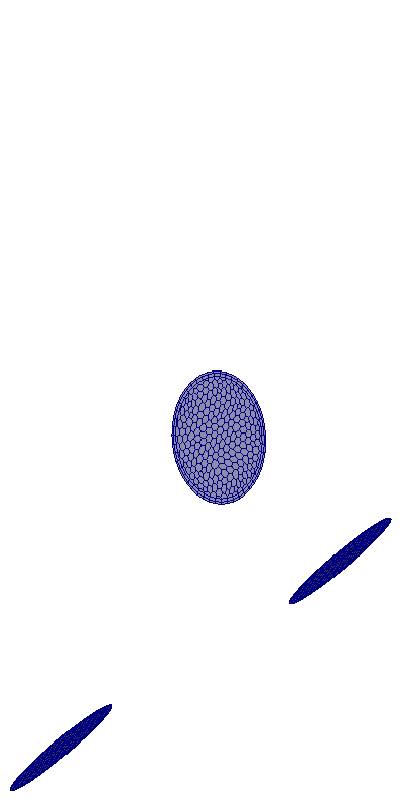
\includegraphics[scale=0.4]{M23out.png} \\
        \hline
        \textcolor{dred}{\texttt{inlet.stl}} & \textcolor{dgreen}{\texttt{fixed.stl}} & \texttt{wall.stl} &  \textcolor{dblue}{\texttt{outlet.stl}} \\
        \hline
        \textcolor{dred}{\texttt{inlet1}}, \textcolor{dred}{\texttt{inlet2}} &  
        \textcolor{dgreen}{\texttt{fixed1}} \textcolor{gray}{\texttt{[inlet1]}},  \textcolor{dgreen}{\texttt{fixed2}} \textcolor{gray}{\texttt{[inlet2]}} ,
        \textcolor{dgreen}{\texttt{fixed3}} \textcolor{gray}{\texttt{[outlet1]}},  \textcolor{dgreen}{\texttt{fixed4}} \textcolor{gray}{\texttt{[outlet2]}},
        \textcolor{dgreen}{\texttt{fixed5}} \textcolor{gray}{\texttt{[outlet3]}},  \textcolor{dgreen}{\texttt{fixed6}}
        & \texttt{wall.stl} & \textcolor{dblue}{\texttt{outlet.stl}} \\
        \hline
    \end{tabular}
    \caption{Geometric data in STL format.}\label{tab:stlData1}
\end{table}


%\begin{figure}[H]
%\centering
%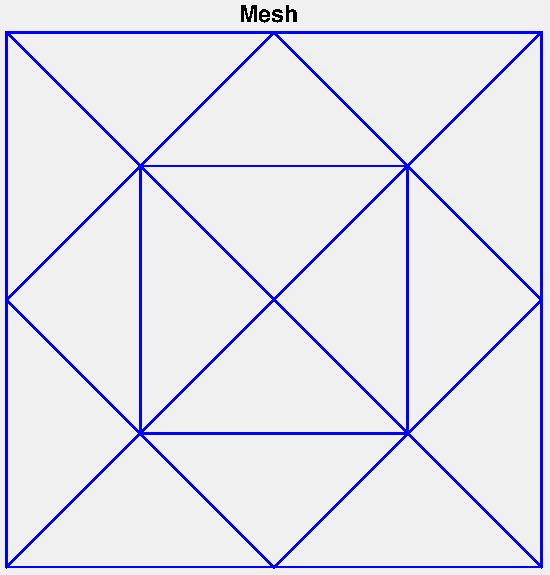
\includegraphics[width=\textwidth]{2}
%\caption{Geometry data in STL format..}
%\end{figure}
%
%\begin{figure}[H]
%\centering
%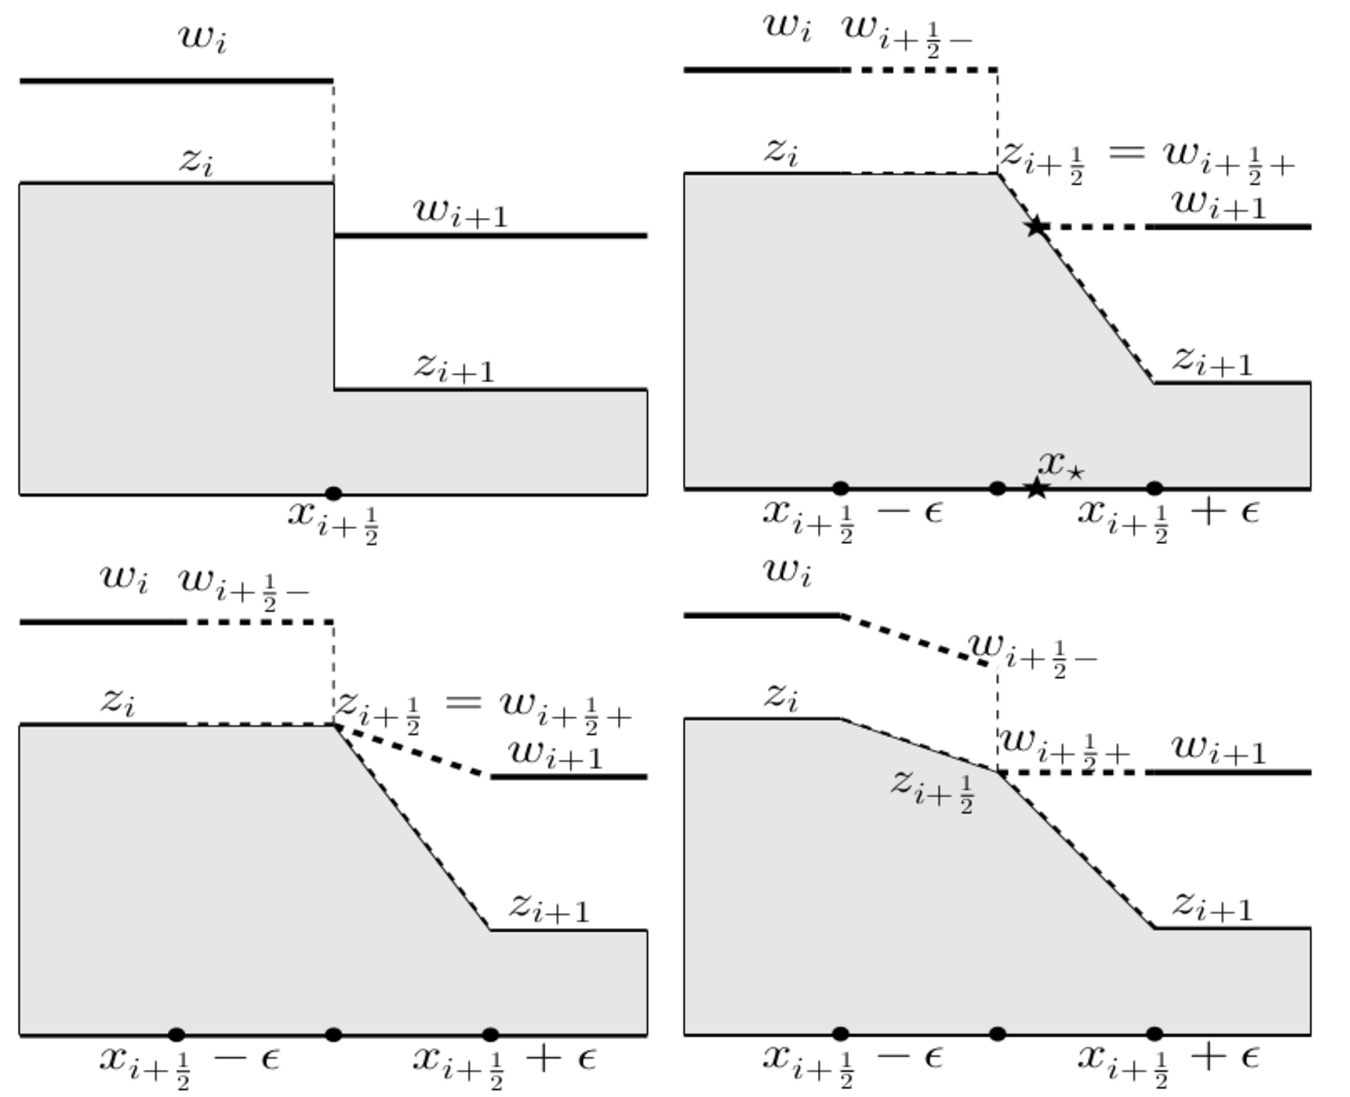
\includegraphics[width=\textwidth]{3}
%\caption{Geometry data in STL format.}
%\end{figure}

\section{Modeling of the inflow/outflow areas}
The following preparation serves to represent the modeling of an application with regard to the surface geometries of the inflow areas and the outflow areas.

\subsection{Inflow areas}
Any number of inlet flow areas can be defined.

One inlet flow area can also consist of several unconnected geometries.

The characteristic of an inflow area is not the shape or topology but the physical properties, such as incoming flow velocity.
\begin{itemize}
    \item Therefore, an application with the same inflow velocity can also be modeled with an inflow area (left graph in Fig. 2.2).
    \item If there are different inflow velocities in the application, different inflow ranges must be defined (right graph in Fig. \ref{fig:multiInlet}).
\end{itemize}

\begin{figure}[htbp]
    \centering
    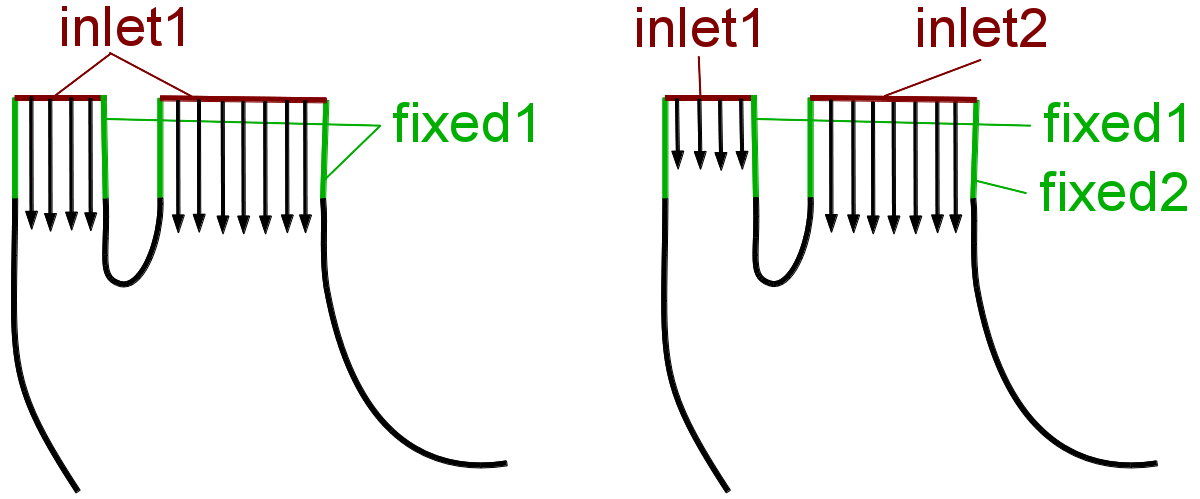
\includegraphics[scale=0.7]{inletMULT.png}   
    \caption{Inflow areas.}
    \label{fig:multiInlet}
\end{figure}

\subsection{Outflow area}
Any number of outflow ranges can be defined.

Analogous to the definition of the inflow areas, the outflow areas will be determined on the basis of the physical properties.

In previous applications, however, the ``do nothing'' boundary condition was always used.

The division into different air outflow areas is also relevant if different air outflow profiles are required.

Fig. \ref{fig:multiOutlet} shows the two optimization variants for a uniform outflow ($\mathcal{J}_1$) is illustrated.

\begin{figure}[htbp]
    \centering
    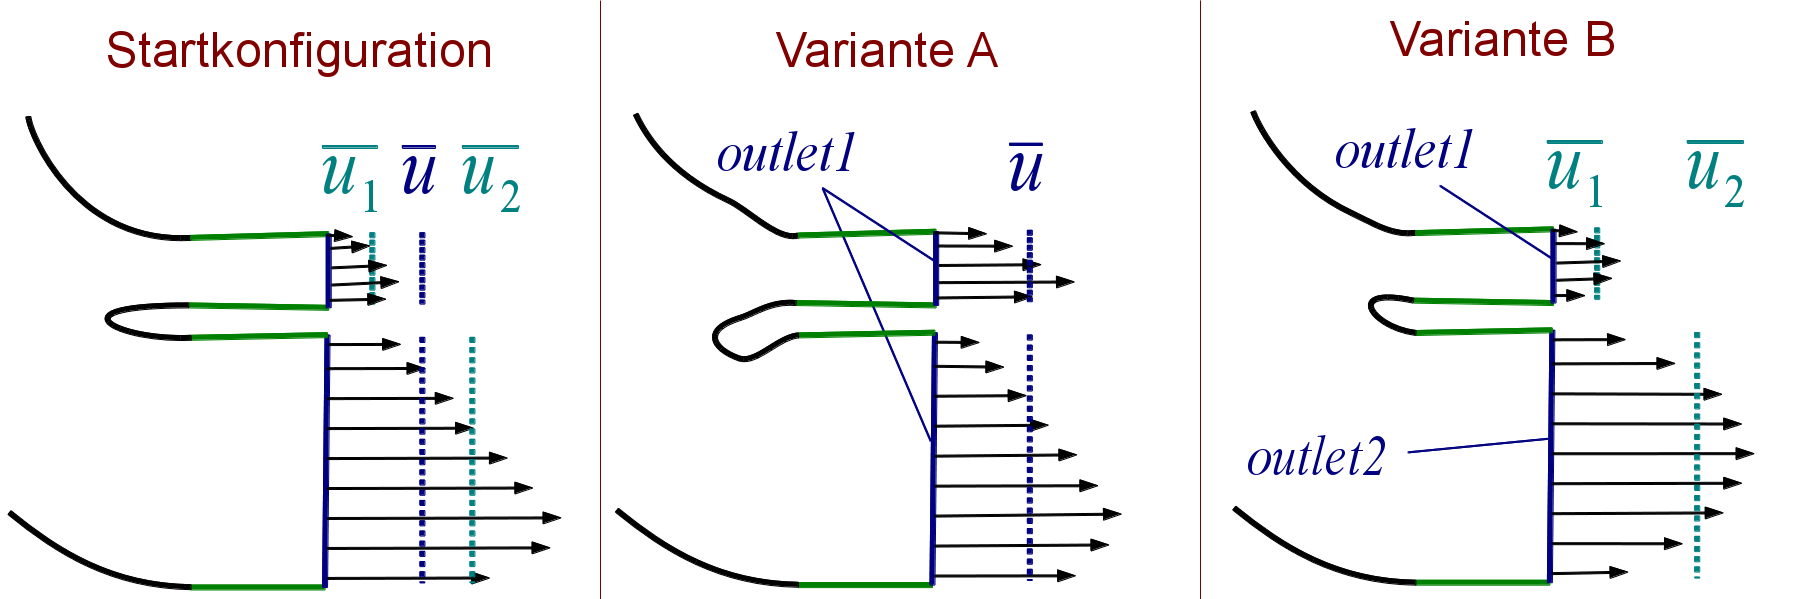
\includegraphics[scale=0.7]{outletMULT.png}   
    \caption{Left: Start. Middle: Optimization $\mathcal{J}_1|_{\Gamma_{\rm out}^1\cup\Gamma_{\rm out}^2}$. Right: Optimization $\gamma_1\mathcal{J}_1|_{\Gamma_{\rm out}^1} + \gamma_2\mathcal{J}_1|_{\Gamma_{\rm out}^2}$.}
    \label{fig:multiOutlet}
\end{figure}

\section{Custom inflow profile}
If an inflow profile is specified, the corresponding entry in the parameter \verb|velocity_massflow| must be set to 0 and a file \verb|velocity_inletI.csv| with $I = \{0,1,2,\ldots\}$ must be specified in the order of the test calculation.\footnote{HN: ?}

If in the example \textit{M23} a profile is specified at the second inflow area, \verb|velocity_massflow = 2(36.5, 0)| will be set and a file \verb|velocity_inlet2.csv| will be created.

\section{Initial geometry topology optimization}
For topology optimization, the largest possible initial geometry should be specified.

Figure \ref{fig:initialTopo} shows an initial geometry for the application example \textit{clean air pipe} (RLR).

\begin{figure}[htbp]
    \centering
    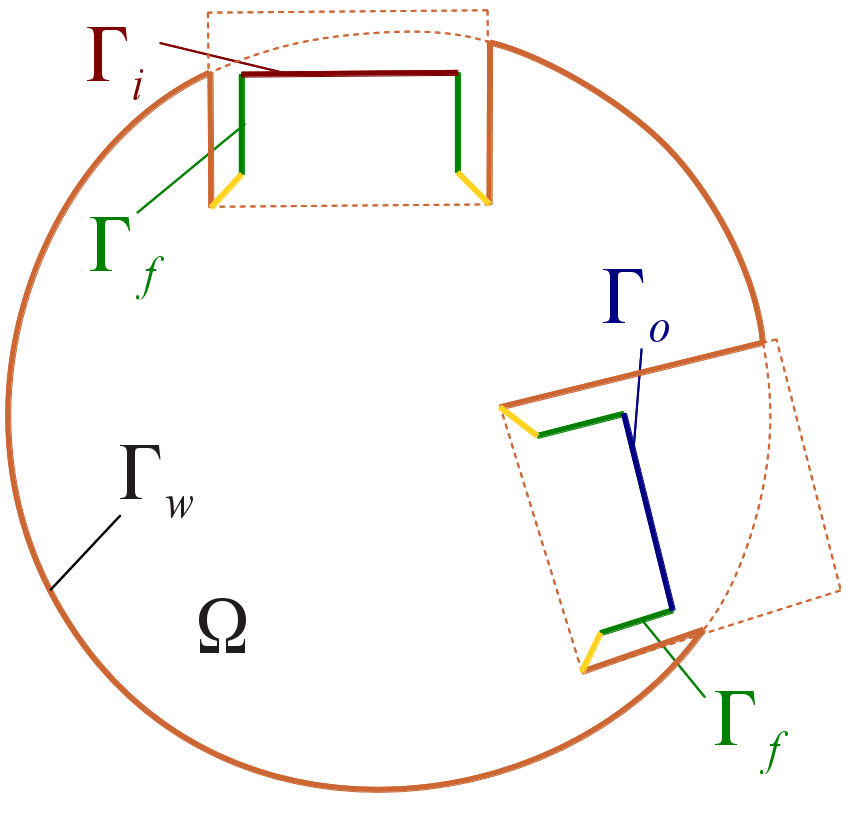
\includegraphics[height=5cm]{TopoStartgeometrieSkizze.png}
    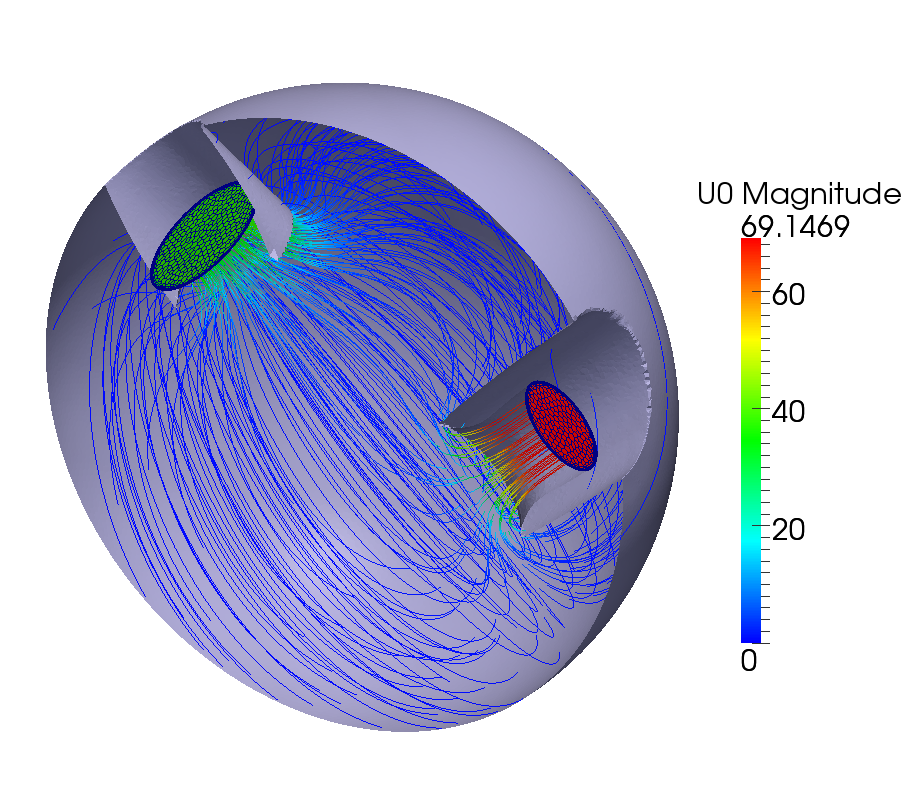
\includegraphics[height=5.5cm]{TopoStartgeometrie.png}
    \caption{Anfangsgeometrie Topologieoptimierung RLR.}
    \label{fig:initialTopo}
\end{figure}

%------------------------------------------------------------------------------%

\chapter{Parameters and their Meanings}

In addition to the geometry data, the parameter file \verb|parameter_sg|\footnote{HN changes to \texttt{parameterDict} and stores it in the \texttt{constant} folder.} must be created.

The parameters it contains are explained in this chapter.

The parameters are inserted in the Java scripts \texttt{mbmw3.java}, \texttt{solvePrimal.java} and \texttt{solveAdjoint.java}.

If changes are to be made in the Star-CCM+ usage, these three files in the \texttt{initialSG} folder must be adjusted.

The parameters relevant for OpenFOAM are stored in \texttt{system/fvSolution} after the setup routine has been called.

\begin{table}[!htbp]]
\centering
\begin{tabular}{|l|c|c|c|c|p{6cm}|}
\hline 
\cellcolor{light-gray}\textbf{Parameter name} & \cellcolor{light-gray}\textbf{Default value} & \cellcolor{light-gray}\textbf{Admissibility} & \cellcolor{light-gray}\textbf{RLR} & \cellcolor{light-gray}\textbf{M23} & \cellcolor{light-gray}\textbf{Description} \\ 
\hline 
\verb|install_location| &  &  &  &  & Path of the  Star-CCM+ bin File to start Star-CCM+. \\ 
\hline 
\texttt{prozessNumber} & 2 & $[1,100]$ & 2 & 2 & Number of processors with parallelization in  Star-CCM+.\\ 
\hline 
\end{tabular} 
\caption{Parameter Star-CCM+.}
\end{table}
HN changed \texttt{prozessNumber} to \texttt{nProcessors}.

\section{Grid generation}
In Star-CCM+ a polyhedron mesh is created.

The mesh fineness can be adjusted using the reference value for the cell size \verb|base_size|.

The number of inlets and outlets and the number of optional fixed surfaces must be specified (\texttt{numInlet}, \texttt{numOutlet}, \texttt{numFixed}).

The mesh quality for mesh generation can be increased using the \verb|mesh_opt_cycles| and \verb|mesh_quality_treshold| parameters.

Near the wall, layers are to be used whose size and number are defined by the \verb|num_layer_wall|, \verb|thick_layer| and \verb|layer_stretch| parameters.

To prevent backflow on the outflow geometry (``do-nothing'' boundary condition), an additional extrusion geometry is usually required.

The adjustment of length and discretization can be defined with the parameters \verb|extrude_... parameters|.

Based on the surfaces in Star-CCM+, the mesh is locally refined in Star-CCM+. 

If this refinement is not is to be executed, the parameter \verb|grid_local_refinement| must be set to 0.

\begin{table}[!htbp]]
    \begin{tabular}{|l|r|r|r|r|r|p{5cm}|}
        \hline 
        \cellcolor{light-gray}\textbf{Parameter name} & \cellcolor{light-gray}\textbf{Default} & \cellcolor{light-gray}\textbf{Admissibility} & \cellcolor{light-gray}\textbf{RLR} & \cellcolor{light-gray}\textbf{M23} & \cellcolor{light-gray}\textbf{B135} & \cellcolor{light-gray}\textbf{Description} \\ 
        \hline 
        \verb|base_size| & 0.004 & [1e-4,0.1] & 0.004 & 0.03 & 0.04 & Grid fineness: cell size. \\ 
        \hline 
        \texttt{numInlet} & 1 & $\rm\left\{1,2,\ldots,1e3\right\}$ & 1 & 2 & 1 & Number of inflow areas. \\ 
        \hline 
        \texttt{numOutlet} & 1 & $\rm\left\{1,2,\ldots,1e3\right\}$ & 1 & 3 & 1 & Number of outflow areas. \\ 
        \hline 
        \texttt{numFixed} & 0 & $\rm\left\{0,1,\ldots,1e3\right\}$ & 0 & 1 & 0 & Number of optionally fixed geometries. \\ 
        \hline 
        \verb|num_layer_wall| & 2 & $\left[0,6\right]$ & 2 & 3 & 6 & Number of layer layers on the edge. \\ 
        \hline 
        \verb|thick_layer| & 60 & $\left[10,100\right]$ & 80 & 60 & 60 & Thickness of the layer layers in percent (Relative to the neighboring cell size). \\ 
        \hline 
        \verb|layer_stretch| & 1.5 & [1e-3,1e3] & 1.5 & 1.5 & 1.4 & Magnification factor d. Layer layers. \\ 
        \hline 
        \verb|extrude_outlet_length| & 0.05 & [1e-8,1e8] & 0.06 & 0.2 & 1.2 & Length of the extrusion geometry at the outlet. \\ 
        \hline 
        \verb|extrude_outlet_num| & 32 & [1,1e5] & 20 & 10 & 90 & Number of cell layers in the extrusion geometry
        at the outlet. \\ 
        \hline 
        \verb|extrude_outlet_stretch| & 1 & [1e-3,1e3] & 1 & 1 & 1 & Magnification factor d. Layer layers in d. Extrusion geometry at the outlet. \\ 
        \hline 
        \verb|extrude_inlet_length| & 0.025 & [1e-8,1e8] & 0.03 & 0.2 & 0.2 & Length of the extrusion geometry on the inlet. \\ 
        \hline 
        \verb|extrude_inlet_num| & 16 & [1,1e5] & 10 & 10 & 15 & Number of cell layers in the extrusion geometry on the inlet. \\ 
        \hline 
        \verb|extrude_inlet_stretch| & 1 & [1e-3,1e3] & 1 & 1 & 1 & Magnification factor of the layer layers
        in the extrusion geometry on the inlet. \\ 
        \hline 
        \verb|mesh_opt_cycles| & 8 & $\left[1,8\right]$ & 8 & 8 & 8 & Polyhedron grid: quality optimization loops. \\ 
        \hline 
        \verb|mesh_quality_threshold| & 1 & $\left[0,1\right]$ & 1 & 1 & 1 & Polyhedron grid: quality optimization barrier. \\ 
        \hline 
        \verb|grid_local_refinement| & 0 & $\left\{0,1\right\}$ & 0 & 1 & 1 & Local mesh refinement: 0: no, 1: yes. \\ 
        \hline 
        \verb|ext_merge| & 0 & $\left\{0,1\right\}$ & 0 & 1 & 0 & Extrusion geometry with fixed geometries
        unite: 0: no, 1: yes. \\ 
        \hline 
    \end{tabular}
    \caption{Grid generation parameters in  Star-CCM+.}
\end{table}

\section{Model selection and physical settings}
To specify the flow velocity, either a constant inflow velocity in m/s or the mass flow rate in kg/s can be specified: \verb|velocity_massflow_par| = 0 or 1.\footnote{Careful with declaring the physical units in OpenFOAM}

The values are to be specified by the parameter \verb|velocity_massflow|.

The corresponding syntax can be found in Table 5.

Beside the Direct Numerical Simulation (\verb|turb_model| = 0), currently 4 turbulence models can be selected with the parameter \verb|turb_model|.

If other turbulence models prove to be suitable for future software versions, the Java script \texttt{mbmw3.java} must be adapted accordingly.

Furthermore, the following model parameters must be specified in  Star-CCM+:
\begin{verbatim}
inlet_turb_intensity, inlet_visc_ratio, outlet_turb_intensity, outlet_visc_ratio
\end{verbatim}

\begin{table}[!htbp]]
    \begin{tabular}{|l|c|c|c|p{1cm}|c|p{5cm}|}
        \hline 
        \cellcolor{light-gray}\textbf{Parameter name} & \cellcolor{light-gray}\textbf{Default} & \cellcolor{light-gray}\textbf{Admissibility} & \cellcolor{light-gray}\textbf{RLR} & \cellcolor{light-gray}\textbf{M23} & \cellcolor{light-gray}\textbf{B135} & \cellcolor{light-gray}\textbf{Description} \\ 
        \hline 
        \verb|turb_model| & 2 & $\left[0,100\right]$ & 1 & 0 & 4 & 0: DNS, 1: Realiz. k-$\epsilon$ all Y+, 2: Std. k-$\epsilon$ high Y+, 3: RSM all Y+, 4: Realiz. k-$\epsilon$ low Y+. \\ 
        \hline 
        \verb|velocity_massflow_par| & 0 & $\left\{0,1\right\}$ & 0 & 0 & 0 & Inflow: 0: speed, 1: mass flow. \\ 
        \hline 
        \verb|velocity_massflow| & 1(0,1) & [1e-8, 1e8] & 1(36.5) & 2(0.006,
        0.006) & 1(4.3) & Inflow (speed
        or mass flow) \\ 
        \hline 
        \verb|inlet_turb_intensity| & 0.1 & [1e-8,1e8] & 0.1 &  & [1e-8, 1e8] & Turbulent Intensity Inlet. \\ 
        \hline 
        \verb|inlet_turb_length| & 10 & [1e-8,1e8] & 0.1 &  & 10 & Turbulent Length Scale Inlet. \\ 
        \hline 
        \verb|outlet_turb_intensity| & 0.1 & [1e-8,1e8] & 0.1 &  & 0.1 & Turbulent Intensity Outlet. \\ 
        \hline 
        \verb|outlet_turb_length| & 10 & [1e-8,1e8] & 0.1 &  & 10 & Turbulent Length Scale Outlet. \\ 
        \hline 
    \end{tabular}    
    \caption{Parameters for physical models.}
\end{table}

\section{Solver settings for the primary and adjoint equation}
The solvers in Star-CCM+ use a pseudo time step method.

The step size control is to be specified using the Courant-Friedrichs-Lewy number (\texttt{CFLpri}, \texttt{CFLadj}).

Choosing a large number allows the desired solution to be achieved more quickly, but can lead to convergence problems if the choice is too large.

For the adjoint equation a GMRES solver (\texttt{gmresAdj}) with the relevant settings \verb|krylov_dim|, \verb|krylov_accuracy| is available in addition to the standard solver.

As termination criteria the maximum number of iterations (\texttt{iterPri}, \texttt{iterAdj}) and a termination at desired accuracies are used.

The second is achieved when the standard deviation is below the tolerance values (\verb|stop_accuracyPri|, \verb|stop_accuracyAdj|).

E.g., if you choose \verb|stop_sample = 100|, the standard deviation of the last 100 iterations is always calculated.

The primary solver is considered to be out-converged if the desired solution accuracy is achieved before reaching the \texttt{iterPri} iteration.

If the accuracy after \texttt{iterPri} steps is not reached, a smaller step size is chosen for the mesh shift.

It is therefore important to always make sure that \texttt{iterPri} is chosen large enough!

If there are convergence problems of the adjoint solver, set the parameter \verb|adj_order| to 1.

\begin{table}[!htbp]
    \begin{tabular}{|l|c|c|c|c|c|p{6.5cm}|}
        \hline 
        \cellcolor{light-gray}\textbf{Parameter name} & \cellcolor{light-gray}\textbf{Default} & \cellcolor{light-gray}\textbf{Admissibility} & \cellcolor{light-gray}\textbf{RLR} & \cellcolor{light-gray}\textbf{M23} & \cellcolor{light-gray}\textbf{B135} & \cellcolor{light-gray}\textbf{Description} \\ 
        \hline 
        \verb|ccm_solver| & 1 & $\left\{0,1\right\}$ & 1 & 1 & 1 & 1: use of Star-CCM+ solver, 0: Alternative solvers. \\ 
        \hline 
        \texttt{gmresAdj} & 0 & $\left\{0,1\right\}$ & 0 & 0 & 0 & Adjoint solver: 0: without GMRES, 1: with GMRES. \\ 
        \hline 
        \verb|krylov_dim| & 50 & [1,1e5] &  &  &  & Number of Krylov spaces (adj,
        GMRES). \\ 
        \hline 
        \verb|krylov_accuracy| & 1e-12 & $\left(0,1\right)$ &  &  &  & Computational accuracy of Krylov spaces. \\ 
        \hline 
        \texttt{CFLpri} & 4 & $\left[0.1,1000\right]$ & 4 & 3 & 4 & CFL primal. \\ 
        \hline 
        \texttt{CFLadj} & 100 & $\left[0.1,10000\right]$ & 90 & 40 & 90 & CFL adjoint. \\ 
        \hline 
        \verb|stop_accuracyPri| & 1e-12 & $\left(0,1\right)$ & 1e-12 & 1e-12 & 1e-8 & Termination criterion standard deviation: Accuracy primary Solution. \\ 
        \hline 
        \verb|stop_accuracyAdj| & 1e-12 & $\left(0,1\right)$ & 1e-12 & 1e-12 & 1e-12 & Termination criterion standard deviation: Accuracy adjoint Solution. \\ 
        \hline 
        \verb|stop_sample| & 100 & [1,1e5] & 200 & 50 & 50 & Termination criterion standard deviation: Number of to contemplating iterations. \\ 
        \hline 
        \texttt{iterPri} & 2000 & [1,1e4] & 4000 & 2500 & 1200 & Maximum iteration number of the primary Equation after a remeshing. \\ 
        \hline 
        \texttt{iterAdj} & 1000 & [1,1e5] & 3000 & 2000 & 1000 & Maximum iteration number of adjoint Equation after one Remeshing. \\ 
        \hline 
        \verb|adj_order| & 2 & $\left\{1,2\right\}$ & 2 & 2 & 1 & Discretization adjoint order. \\ 
        \hline 
    \end{tabular} 
    \caption{Parameters for the solvers in Star-CCM+.}    
\end{table}

\section{Line search}
In the course of shape optimization we use a step size control based on the mesh quality query and the query for a sufficiently large reduction of the function value.

The rule used is called \textit{Armijo line search} and reads
\begin{align}
\label{Armijo line search}
\mathcal{J}_{12}^\alpha \left(\Omega^{k+1}\right) \le \mathcal{J}_{12}^\alpha \left(\Omega ^k\right) - \mu s_k \left\|\mathcal{DJ} _{12}^\alpha \left(\Omega ^k\right)\right\| _{L^2\left(\Gamma _w^k\right)},
\end{align}
with $0<\mu<1$ and $\Omega ^{k+1} = \mathcal{T}_{D\left(s_k, \Omega^k\right)} \left(\Omega ^k\right)$.
The mapping $\mathcal{T} _{D\left(s_k, \Omega ^k\right) \left(\Omega\right)\left(\boldsymbol{x}\right)} : \mathbb{R}^3 \to \mathbb{R}^3$ is determined based on the shape gradient.

The user must specify a starting step length $s_0$ (\texttt{spStepLength}).

In the case that
the condition \eqref{Armijo line search} is not fulfilled, the step size is reduced by the factor \texttt{spReduceKoeff}.

The reduction of the step size is performed until the step size is smaller than the value \texttt{spLowerBound}.

After that a mesh re-connection is performed.

The weighting $\mu > 0$ (\texttt{linesearchWeight}\footnote{Original: \texttt{linesearchGewicht}}) ensures a sufficiently large step size, which is relevant for the mathematical consideration of the line search.

For numerical applications this parameter should be set rather small.

If you want to force a mesh re-connection after a certain number of iterations, you can use the parameter \verb|remesh_iter|.

Usually, mesh re-connection is not necessary if the mesh is valid.

Therefore, this value was set higher than the maximum number of iterations in the calculations.


\begin{table}
    \begin{tabular}{|l|c|c|c|c|p{7.5cm}|}
        \hline 
        \cellcolor{light-gray}\textbf{Parameter name} & \cellcolor{light-gray}\textbf{Default} & \cellcolor{light-gray}\textbf{Admissibility} & \cellcolor{light-gray}\textbf{RLR} & \cellcolor{light-gray}\textbf{M23} & \cellcolor{light-gray}\textbf{Description} \\ 
        \hline 
        \texttt{spStepLength} & 2.0e-6 & $\left[0,1\right]$ & 1e-4 & 1e-2 & Starting step size $s_0$ in the
        Armijo line search 3.1. \\ 
        \hline 
        \texttt{spLowerBound} & 1.0e-8 & $\left[0,1\right]$ & 1e-6 & 1e-5 & Lower bound of the step size. \\ 
        \hline 
        \texttt{spReduceKoeff} & 0.5 & $\left[0,1\right]$ & 0.6 & 0.5 & Reduction factor at Step size control. \\ 
        \hline 
        \texttt{linesearchGewicht} & 1.0e-16 & $\left[0,1\right]$ & 1e-14 & 0 & Weighting $\mu$ in Armijo Line search. \\ 
        \hline 
        \verb|remesh_iter| & 1000 & [1,1e5] & 900 & 10 & Remeshing in every \ldots 10 Force iteration (also if mesh quality is OK). \\ 
        \hline 
    \end{tabular} 
    \caption{Line search parameters in OpenFOAM.}
\end{table}

\section{Termination criteria for shape optimization}
Table 8 shows the parameters for completing the shape optimization.

The most relevant parameters are maximum number of iterations (\texttt{outerLoopEnd}), the number of remeshings performed (\verb|rem_max|) and the progress in the target functional (\verb|sigma_stop_J|).

\begin{table}[!htbp]]
    \begin{tabular}{|l|c|c|c|c|p{7.5cm}|}
        \hline 
        \cellcolor{light-gray}\textbf{Parameter name} & \cellcolor{light-gray}\textbf{Default} & \cellcolor{light-gray}\textbf{Admissibility} & \cellcolor{light-gray}\textbf{RLR} & \cellcolor{light-gray}\textbf{M23} & \cellcolor{light-gray}\textbf{Description} \\
        \hline 
        \texttt{outerLoopEnd} & 8 & [1,1e5] & 200 & 200 & Maximum number of iterations. \\ 
        \hline 
        \verb|rem_max| & 20 & $\left[1,1000\right]$ & 30 & 30 & Maximum number of performed Remeshings. \\ 
        \hline 
        \verb|rem_num_max| & 8 & $\left[1,1000\right]$ & 30 & 30 & Maximum number of remeshings
        with \verb|rem_tol| distance. \\ 
        \hline 
        \verb|rem_tol| & 2 & $\left[0,100\right]$ & 2 &  & Distance tolerance for remeshing. \\ 
        \hline 
        \verb|sigma_stop_J| & 50 & $\left[0,100\right]$ & 100 & 100 & Termination criterion: progress in \% in the target functional J. Notation: $\sigma$. \\ 
        \hline 
        \verb|sigma_stop_DJ| & 50 & $\left[0,100\right]$ & 100 & 100 & Termination criterion: progress in \% in the $L^2$-norm of the shape gradient. Notation: $\sigma _d$. \\ 
        \hline 
    \end{tabular}    
    \caption{Termination criteria of shape optimization in OpenFOAM.}
\end{table}

\section{Shape optimization: Cost functional}

\subsection{Uniform outflow and total pressure loss}
Shape optimization can be carried out with regard to achieving a uniform outflow and minimizing the total pressure loss.

The \textit{discrete cost functional} with regard to uniform outflow is
\begin{align}
\label{discrete cost functional J1}
\mathcal{J}_1 = \frac{1}{\bar{v}} \left(\frac{1}{A}\sum_{k\in\Gamma_{\rm out}} ({\bf v}_k\cdot{\bf n}_k - \bar{v})^2 A_k\right)^{1/2},
\end{align}
with
\begin{align}
\bar{v} = \frac{1}{A}\sum_{j\in\Gamma_{\rm out}} {\bf v}_j\cdot{\bf n}_jA_j,
\end{align}
where $A = |\Gamma_{\rm out}|$.

The discrete cost functional with regard to minimizing the total pressure loss is
\begin{align}
\label{discrete cost functional J2}
\mathcal{J}_2 = \left|\frac{\sum\limits_{k\in\Gamma_{\rm in}} \left(p_k + \frac{\rho_k}{2}({\bf v}_k\cdot{\bf v}_k)\right){\bf v}_k\cdot(-{\bf n}_k)A_k}{\sum\limits_{k\in\Gamma_{\rm in}} {\bf v}_k\cdot(-{\bf n}_k)A_k}\right| - \left|\frac{\sum\limits_{k\in\Gamma_{\rm out}} \left(p_k + \frac{\rho_k}{2}({\bf v}_k\cdot{\bf v}_k)\right){\bf v}_k\cdot{\bf n}_kA_k}{\sum\limits_{k\in\Gamma_{\rm out}} {\bf v}_k\cdot{\bf n}_kA_k}\right|.
\end{align}
With ${\bf v}_k$ we denote the velocity vector at the finite surface with index $k$.

The pressure $p_k$ and the density $\rho_k$ is also evaluated at the finite surface with index $k$.

In order to keep the notation simple, we denote the index set of all surface pieces at the inflow and outflow geometry with $\Gamma_{\rm in}$ and $\Gamma_{\rm out}$ respectively.

The surface dimension of a finite surface is designated with $A_k$.

The outwardly directed unit normal vector is designated ${\bf n}_k$.

The unit normal vector ${\bf n}_k$ on $\Gamma_{\rm in}$ is oriented against the main flow direction.

This results in the mixed objective functional:
\begin{align}
\label{mixed cost functional}
\mathcal{J}_{12}({\bf v}(\Omega) = (1 - \gamma)\mathcal{J}_1({\bf v}(\Omega)) + \gamma\rho\mathcal{J}_2({\bf v}(\Omega)),
\end{align}
with $\gamma\in[0,1]$ and
\begin{equation*}
\rho = \left\{\begin{split}
& \frac{\|\partial\mathcal{J}_1({\bf v}(\Omega^0))\|_{L^2(\Gamma_{\rm wall}^0}}{\|\partial\mathcal{J}_2({\bf v}(\Omega^0))\|_{L^2(\Gamma_{\rm wall}^0}} &\mbox{ if } \gamma\in(0,1),\\
& 1 &\mbox{ if } \gamma\in\{0,1\},
\end{split}\right.
\end{equation*}
with the \textit{weighting parameter} $\gamma$ (\verb|dp_J12|).

\begin{figure}[htbp]
    \centering
    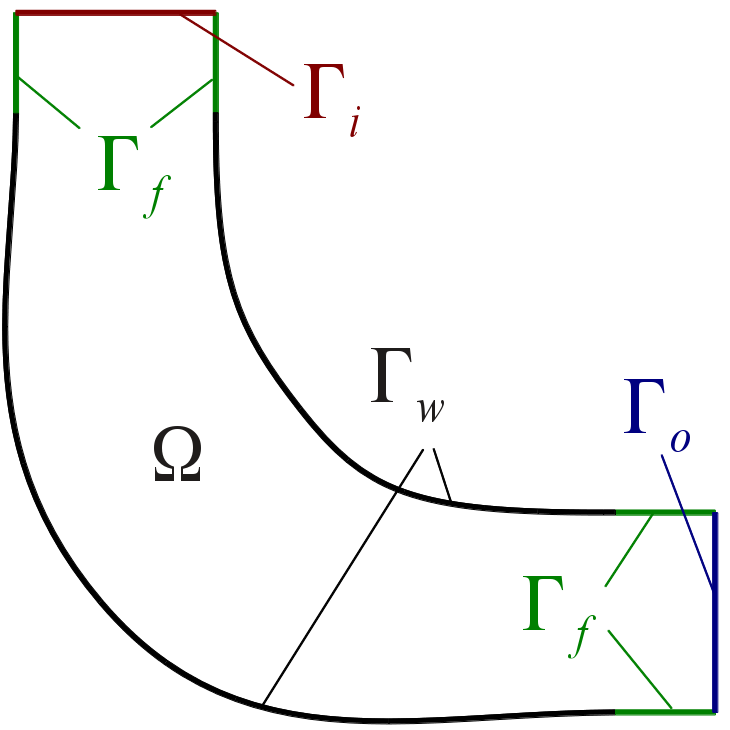
\includegraphics[scale=0.7]{geometrie_skizze_noInterface.png}
    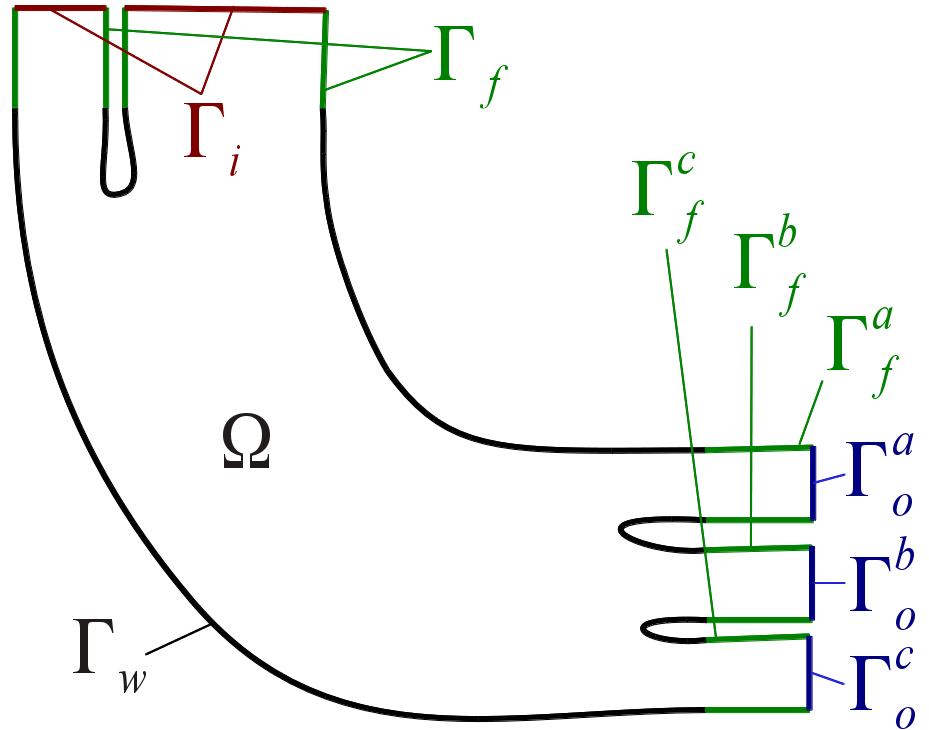
\includegraphics[scale=0.7]{geometrie_skizze_MultOutlet.png}
    \caption{Sketch of $\Omega$ with designation of the parts of the surface.}
    \label{Sketch_extrusion}
\end{figure}

The parameter \verb|gnu_plot_visual| and \verb|gnu_plot_visual_i| are used for the graphical representation of the target function values.

If this option is selected, the graphics appear during the shape optimization and are stored in the test run folder under \verb|Function_values_J1.ps|, \verb|Function_values_J2.ps| and \verb|Function_values_J12.ps|.

\begin{table}[htbp]
    \centering
    \begin{tabular}{|c|c|c|c|c|c|}
        \hline
        \cellcolor{light-gray}\textbf{Parameter name} & \cellcolor{light-gray}\textbf{Default} & \cellcolor{light-gray}\textbf{Admissibility} & \cellcolor{light-gray}\textbf{RLR} & \cellcolor{light-gray}\textbf{M23} & \cellcolor{light-gray}\textbf{Description} \\
        \hline
        \verb|dp_J12| & 0.5 & $[0,1]$ & 0.5 & 0.5 & Weighting parameters $\gamma$ between $\mathcal{J}_1$ and $\mathcal{J}_2$. \\
        \hline
        \verb|dp_J1| & 1(0) & $\sum$\verb|dp_J1|$\in[0,1]$ & 1(0) & 3(0.25,0.25,0.25) & Weighting parameter $\gamma_i$ concerning $\mathcal{J}_1$. \\
        \hline
        &  &  &  &  &  \\
        \hline
        &  &  &  &  &  \\
        \hline
    \end{tabular}
\end{table}



%------------------------------------------------------------------------------%

\chapter{Initialization and Calculation}

%------------------------------------------------------------------------------%

\chapter{Data evaluation and visualization}

%------------------------------------------------------------------------------%


%------------------------------------------------------------------------------%

\newpage
\begin{thebibliography}{99}
\bibitem{Handbuch zur Software} Michael Hinterm\"uller, Karl. Knall, MMag. M. Kanitsar. \textit{Handbuch zur Software: ``Form- und Topologieoptimierung''}, Software-Version: 1612.

\bibitem{Benchmark} Naomi Auer, Michael Hinterm\"uller, Karl Knall. \textit{Part VIII. Benchmark Case for Optimal Shape Design of Air Ducts in Combustion Engines}. In: ROMSOC, \textit{Reports about 8 selected benchmark cases of model hierarchies}, Deliverable number: D5.1, Version 0.1.
\end{thebibliography}
\end{document} 